% Two-column scientific paper (IEEEtran conference class, two-column layout with
% column-width figures and floats placed at column tops so that no gaps remain).
% All numbers come from generated/values.tex, written by `python run_all.py`.
\documentclass[conference,letterpaper]{IEEEtran}
\usepackage{amsmath,amssymb}
\usepackage{graphicx}
\usepackage{booktabs}
\usepackage{balance}
\usepackage[hidelinks]{hyperref}
% PDF metadata (kept in step with REPORTS in reports/build/build_reports.py)
\hypersetup{pdftitle={Reliability-Based Optimisation and Adaptive Operation of a Jacketed Stirred-Tank Cooling Process},
  pdfauthor={Nithin D H},
  pdfsubject={Scientific paper, ESC113M extended project (V3), Department of Chemical Engineering, Indian Institute of Technology Kanpur},
  pdfkeywords={jacketed stirred tank; RK4; Monte Carlo; chance-constrained optimisation; Sobol sensitivity; adaptive operation; simulation study},
  pdfcreator={pdfLaTeX},
  pdfinfo={Institution={Department of Chemical Engineering, Indian Institute of Technology Kanpur}}}
\graphicspath{{figures/}}
\input{generated/values.tex}
\newcommand{\mdot}{\dot m}

\begin{document}

\title{Reliability-Based Optimisation and Adaptive Operation of a Jacketed Stirred-Tank Cooling Process}

\author{\IEEEauthorblockN{Nithin D H}
\IEEEauthorblockA{Department of Chemical Engineering, Indian Institute of Technology Kanpur\\
nithindh23@iitk.ac.in}}

\maketitle

\begin{abstract}
A single-state model of a hot liquid cooled in a stirred tank is extended to coupled liquid and jacket-coolant energy balances with a finite coolant inventory, a heat-transfer coefficient that depends on agitator speed and coolant flow, a saturated coolant actuator and an agitator-plus-pump electricity model. The model is integrated with fourth-order Runge--Kutta and verified against its exact matrix-exponential solution (observed order \vConvOrder). Coolant warming reverses the original model's conclusion: at the reference point the liquid ends at \vTBase\ K instead of \vTOrig\ K and misses a 355 K target. A chance-constrained search on \vNOpt\ Monte Carlo batches, with a lower-confidence-bound rule and validation on \vNVal\ independent batches, selects \vRecRpm\ rpm at the 0.50 kg/s pump limit: P(pass)~=~\vRecPass\,\% (lower bound \vRecLB\,\%) at \vRecE\ kWh per batch. In simulation, a policy that estimates the heat-transfer conductance from ten minutes of noisy temperature data reaches \vAdPass\,\% at \vAdMeanE\ kWh, but it is more sensitive than the fixed setting to the assumed heat-transfer closure.
\end{abstract}

\begin{IEEEkeywords}
jacketed vessel, Runge--Kutta, Monte Carlo, chance-constrained optimisation, Sobol sensitivity, soft sensor
\end{IEEEkeywords}

\section{Introduction}
The original ESC113M project modelled a perfectly mixed liquid cooled by a jacket held at 300 K, \(M_LC_{p,L}\,dT_L/dt = -UA(T_L - T_c)\), and solved it with RK4. That model treats the jacket as an infinite sink and has no operating variables, so it cannot say which agitation and coolant flow to use. This work keeps the same tank (500 kg, \(A = 2\) m\textsuperscript{2}, \(U_{ref} = 150\) W/(m\textsuperscript{2}K), 370 K initial temperature, 1800 s horizon) and asks: \emph{which agitator speed \(N\) and commanded coolant flow \(\mdot_{cmd}\) reach \(T_L \le 355\) K by 1800 s at minimum auxiliary electricity, and how reliably?} The contributions are a verified two-state model, a reduced-order design equation, a validated reliability-based optimum under a physical pump limit, an adaptive policy, and a model-form stress test.

\section{Mathematical Model and Methodology}
\subsection{Coupled energy balances}
With \(T_J\) the well-mixed jacket temperature and \(\mdot\) the delivered coolant flow,
\begin{align}
M_LC_{p,L}\,\dot T_L &= -UA\,(T_L - T_J), \label{eq:l}\\
M_JC_{p,C}\,\dot T_J &= UA\,(T_L - T_J) + \mdot C_{p,C}(T_{in} - T_J), \label{eq:j}\\
U &= U_{ref}\,(N/N_{ref})^{0.25}\,(\mdot/\mdot_{ref})^{0.33}, \label{eq:u}
\end{align}
with \(M_J = 10\) kg, \(T_{in} = 300\) K and reference values 300 rpm and 0.20 kg/s. The exponents in (\ref{eq:u}) are assumptions. The pump delivers at most \(\mdot_{max} = 0.50\) kg/s, and a flow loop with a 5\,\% proportional error is modelled as a saturated actuator,
\begin{equation}
\mdot = \min\left[\mdot_{max},\ \mdot_{cmd}(1 + 0.05z)\right],\quad z \sim \mathcal N(0,1), \label{eq:act}
\end{equation}
so that \vFracAtCap\,\% of batches commanded at 0.50 kg/s receive exactly the pump limit. Agitator power is \(N_P\rho n^3D^5/\eta_{ag}\) (\(N_P = 5\), \(D = 0.3\) m) and pump power \(\Delta P\,\mdot/(\rho\eta_p)\) with \(\Delta P \propto \mdot^2\), evaluated at the delivered flow. The objective is the auxiliary electricity \(E = \int (P_{ag} + P_{pump})\,dt\); chiller energy is not included.

\subsection{Reliability-based design}
The uncertain inputs are \(U_{ref} \sim \mathcal N(150, 15^2)\), \(M_J \sim \mathcal N(10, 1)\), \(T_0 \sim \mathcal N(370, 1)\) and \(z\). The design problem is \(\min \mathbb E[E]\) s.t.\ \(\Pr[T_L(t_f) \le 355\ \mathrm K] \ge 0.95\). It is solved as a sample-average approximation~\cite{b3} on an optimisation set (OPT, \(n = \vNOpt\)) with a margin: the one-sided 95\,\% Wilson lower bound~\cite{b4} of the sample pass fraction must reach 95\,\%, i.e.\ \(\hat p \ge \vPReqOpt\,\%\). Under common random numbers the pass fraction is monotone in \(N\), so the minimum speed at each flow is found exactly by bisection. The speed is then rounded up to a 5 rpm setpoint and validated once on an independent set (VAL, \(n = \vNVal\)) whose seed was never examined during development. A design that failed VAL would be modified by a pre-declared rule and re-validated on a second fresh set; none needed it.

\subsection{Adaptive measure-then-set policy}
Phase 1 runs at \(N_1\) for \(t_{obs}\) while \(T_L\) and \(T_J\) are logged every 10 s with 0.1 K noise. A soft sensor fits straight lines to both temperatures and estimates \(\hat Q = -M_LC_{p,L}\,\dot T_L\), \(\widehat{UA} = \hat Q/(T_L - T_J)\) and \(\widehat{\mdot C_p}\). Phase 2 uses the lowest speed whose prediction reaches \(355 - \delta\) K by \(t_f\), up to a cap of 600 rpm. \(N_1\), \(t_{obs}\) and \(\delta\) are chosen on a separate calibration set (CAL); \(\delta\) is rounded up to 0.05 K by a rule fixed before validation.

\section{Numerical Implementation and Verification}
RK4 with \(\Delta t = 1\) s is used for every deterministic trajectory. For constant settings, (\ref{eq:l})--(\ref{eq:j}) are linear, and \(e^{\mathbf Mt}\) has a closed form for the \(2\times2\) matrix with distinct real eigenvalues. This exact solution~\cite{b6} verifies RK4 and evaluates \(T_L(1800\ \mathrm s)\) for large Monte Carlo sets. The RK4 trajectory error against it scales with order \vConvOrder\ and is \(\vErrDtOne\) K at 1 s, well inside the stability limit of \vStabRec\ s set by the fast jacket mode. The first law closes to \vEBResSimp\ J with Simpson quadrature. An independent implementation in MATLAB syntax, executed in \vOctRuntime, reproduces the deterministic results exactly.

\section{Results and Discussion}
\subsection{Coolant-side resistance}
Fig.~\ref{fig:orig} compares the models at 300 rpm and 0.20 kg/s. The jacket warms to \vPeakTJBase\ K, and the liquid ends \vTBaseGap\ K warmer than the original model predicts, which reverses the pass/fail verdict. With a quasi-steady jacket the two resistances add in series, \(1/UA_{eff} = 1/UA + 1/\mdot C_{p,C}\). This gives \(UA_{eff} = \vUAEffBase\) W/K and reproduces the full model to within \vRomErrBase\ K. Requiring \(T_L(t_f) = 355\) K gives \(UA_{eff,req} = M_LC_{p,L}\ln[(T_0-T_{in})/(T_t-T_{in})]/t_f = \vUAEffReq\) W/K. No agitation speed can therefore succeed below \(\mdot = \vMinFlow\) kg/s.

\begin{figure}[!t]
\centering
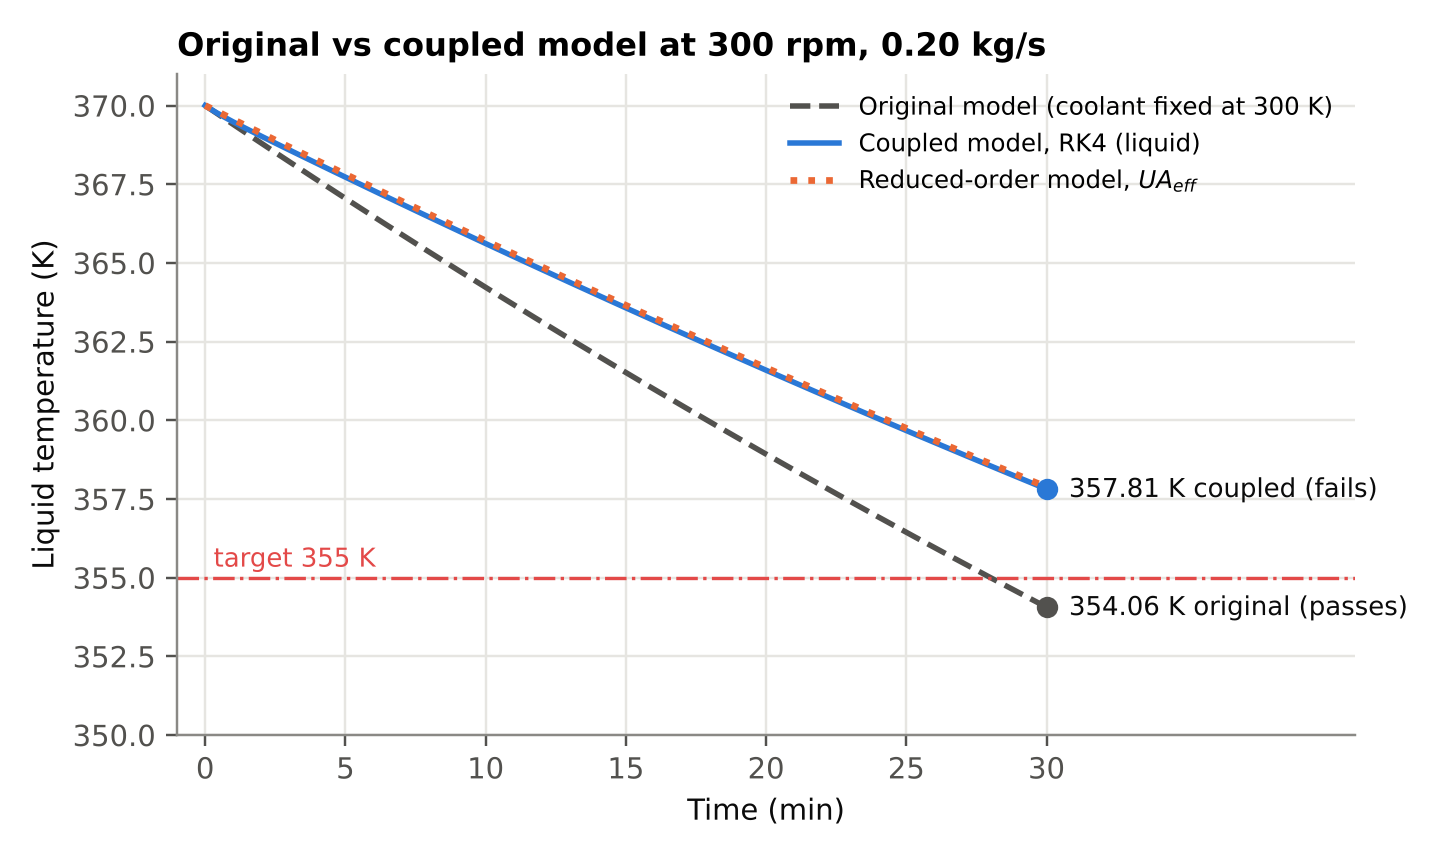
\includegraphics[width=\columnwidth]{model_comparison/original_vs_coupled.png}
\caption{Original constant-coolant model, coupled RK4 model and the series-resistance reduced model at the reference point.}
\label{fig:orig}
\end{figure}

\section{Optimisation and Reliability Findings}
\subsection{Deterministic and reliability-based optimum}
The deterministic minimum-energy point lies on the pump limit, at \vNomRpm\ rpm and \vNomE\ kWh, because agitator power grows as \(N^3\) while \(U\) grows only as \(N^{0.25}\) (Fig.~\ref{fig:window}). The closed-form boundary from \(UA_{eff,req}\) overlays the simulated one. Under uncertainty, however, only \vNomPass\,\% of batches reach the target at that point (Table~\ref{tab:designs}). The chance-constrained optimum on OPT is \vCCRpm\ rpm. Rounded to \vRecRpm\ rpm, it passes \vRecPass\,\% of the VAL batches (95\,\% CI \vRecLo--\vRecHi\,\%) at \vRecE\ kWh. Enforcing the pump limit removes the impossible high-flow batches of the earlier version, so the earlier 285 rpm recommendation now falls short (\vVTwoRecPass\,\%). The Octave implementation, with different random numbers, selects the same setpoint. Fig.~\ref{fig:frontier} shows the price of reliability. Every optimum sits at the pump limit, and going from 90\,\% to 99\,\% reliability multiplies the energy by \vFrRatioB. Sobol indices~\cite{b2} at the recommended point attribute \vSobOneU\,\% of the variance of \(T_L(t_f)\) to \(U_{ref}\), \vSobOneTZero\,\% to \(T_0\), \vSobOneFlow\,\% to the flow error and nothing to \(M_J\).

\begin{table}[!t]
\centering
\caption{Designs on the independent validation set (\(n = \vNVal\); delivered-flow model)}
\label{tab:designs}
\footnotesize
\setlength{\tabcolsep}{4pt}
\input{generated/tab_paper_designs.tex}
\end{table}

\begin{figure}[!t]
\centering
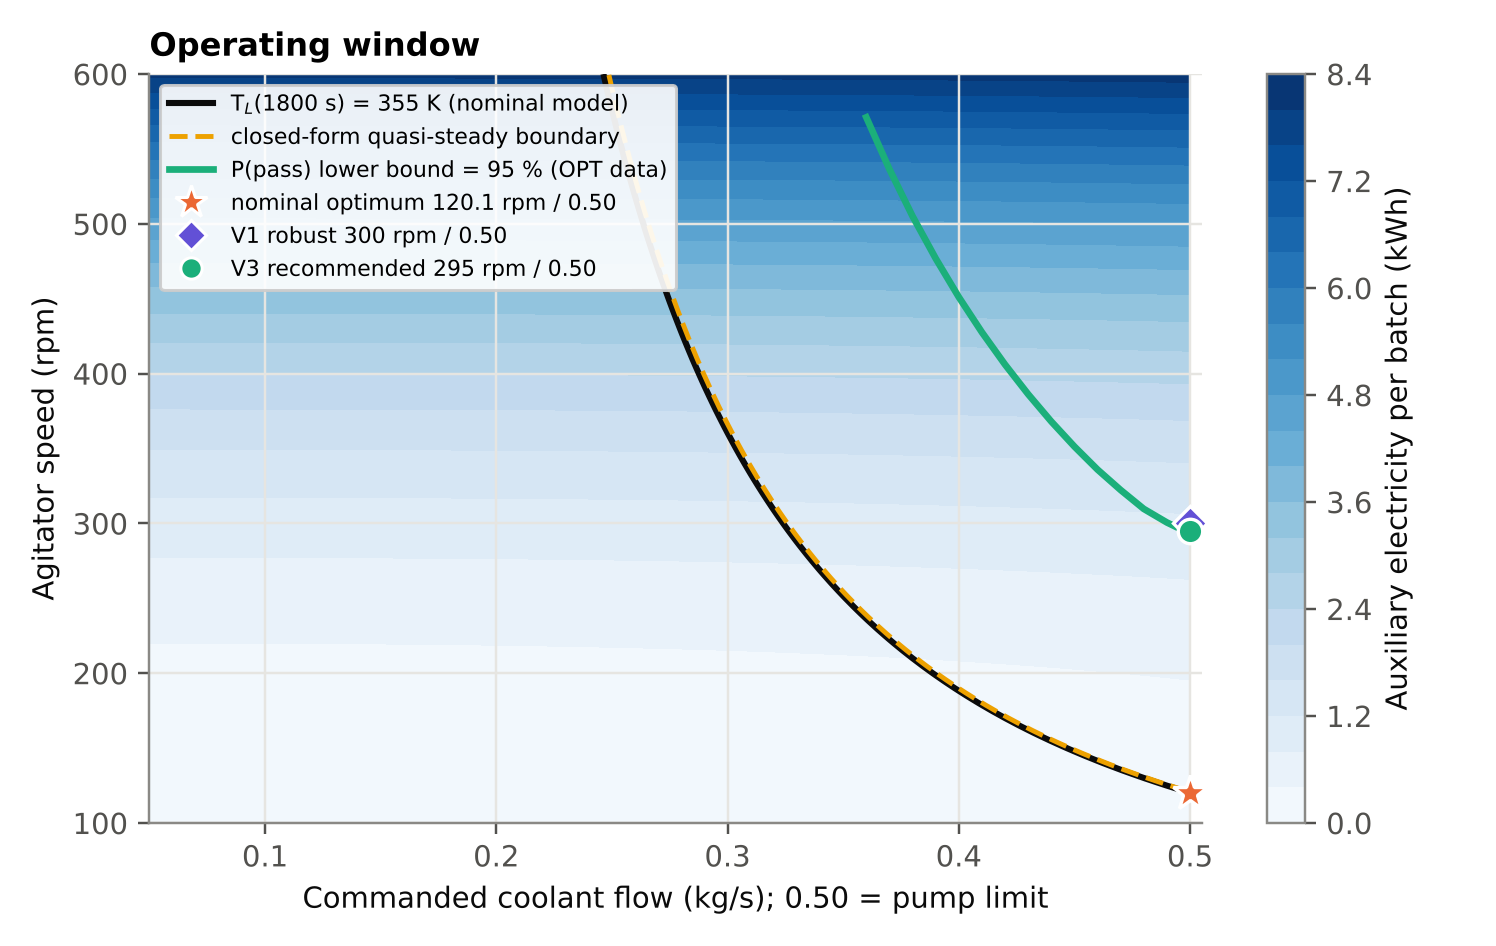
\includegraphics[width=\columnwidth]{optimization/operating_window.png}
\caption{Operating window: auxiliary electricity per batch, the nominal 355 K boundary (simulated and closed-form) and the 95\,\% reliability boundary from the optimisation set.}
\label{fig:window}
\end{figure}

\begin{figure}[!t]
\centering
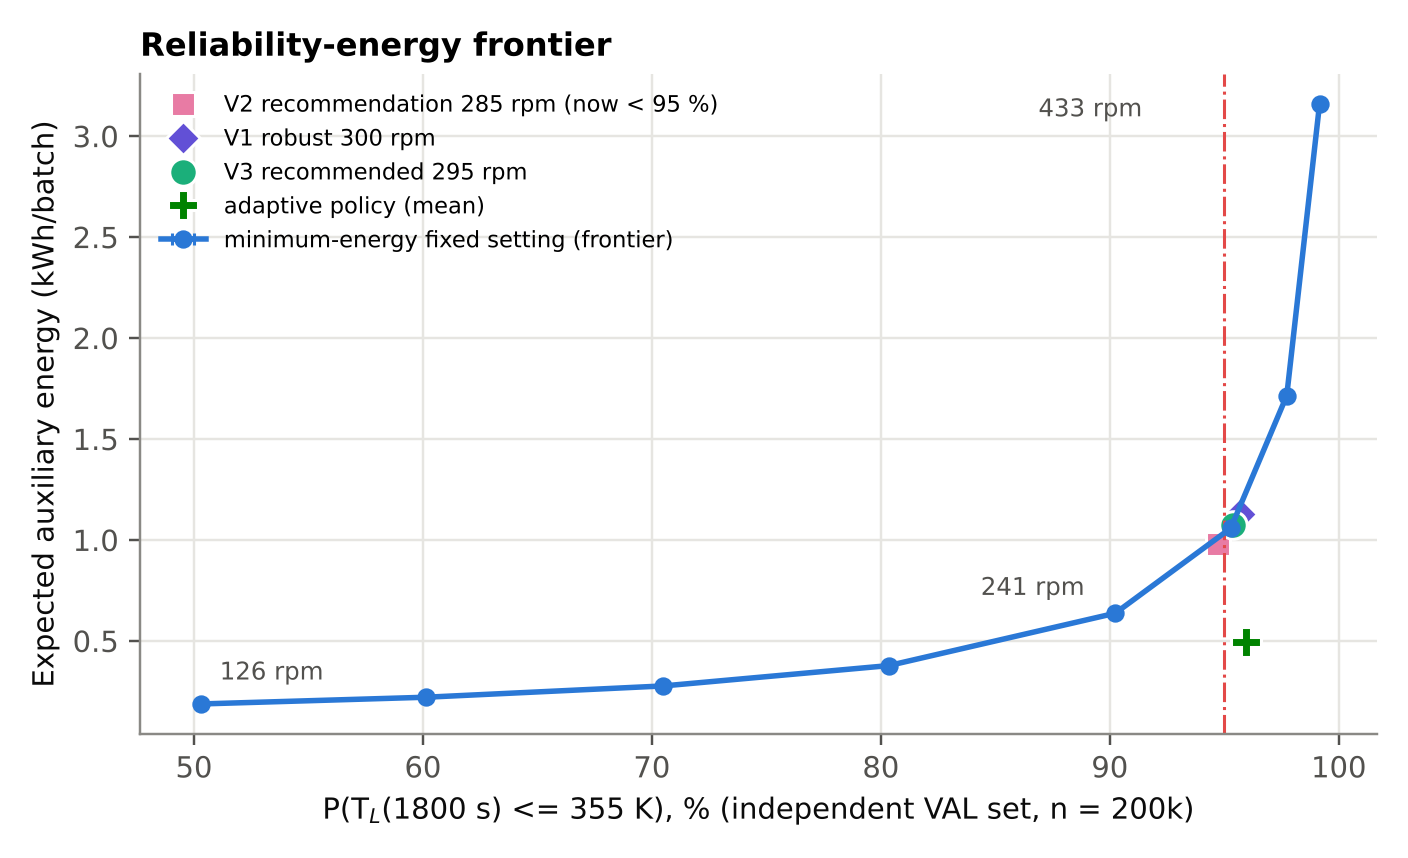
\includegraphics[width=\columnwidth]{optimization/reliability_energy_frontier.png}
\caption{Minimum expected auxiliary electricity for each validated pass probability, with the earlier designs and the adaptive policy.}
\label{fig:frontier}
\end{figure}

\subsection{Adaptive operation}
The CAL search selects \(N_1 = \vAdRpmOne\) rpm and \(t_{obs} = \vAdTobs\) s, with a calibrated margin of \vAdDeltaCal\ K rounded to \(\delta = \vAdDelta\) K. The soft sensor recovers \(UA\) to within \vAdUAErr\,\% (one standard deviation). Validated once on VAL, the policy passes \vAdPass\,\% of batches (95\,\% CI \vAdLo--\vAdHi\,\%, lower bound \vAdLB\,\%) at a mean of \vAdMeanE\ kWh, \vAdSave\,\% below the fixed setting (Fig.~\ref{fig:adaptive}); the Octave replication gives \vOctAdPass\,\%. The energy distribution has a long tail: the median is \vAdMedE\ kWh, but \vAdCap\,\% of batches reach the 600 rpm cap and the 99th percentile is \vAdPNNE\ kWh. These are simulation results with assumed sensor noise; the policy has not been tested on a plant.

\begin{figure*}[!t]
\centering
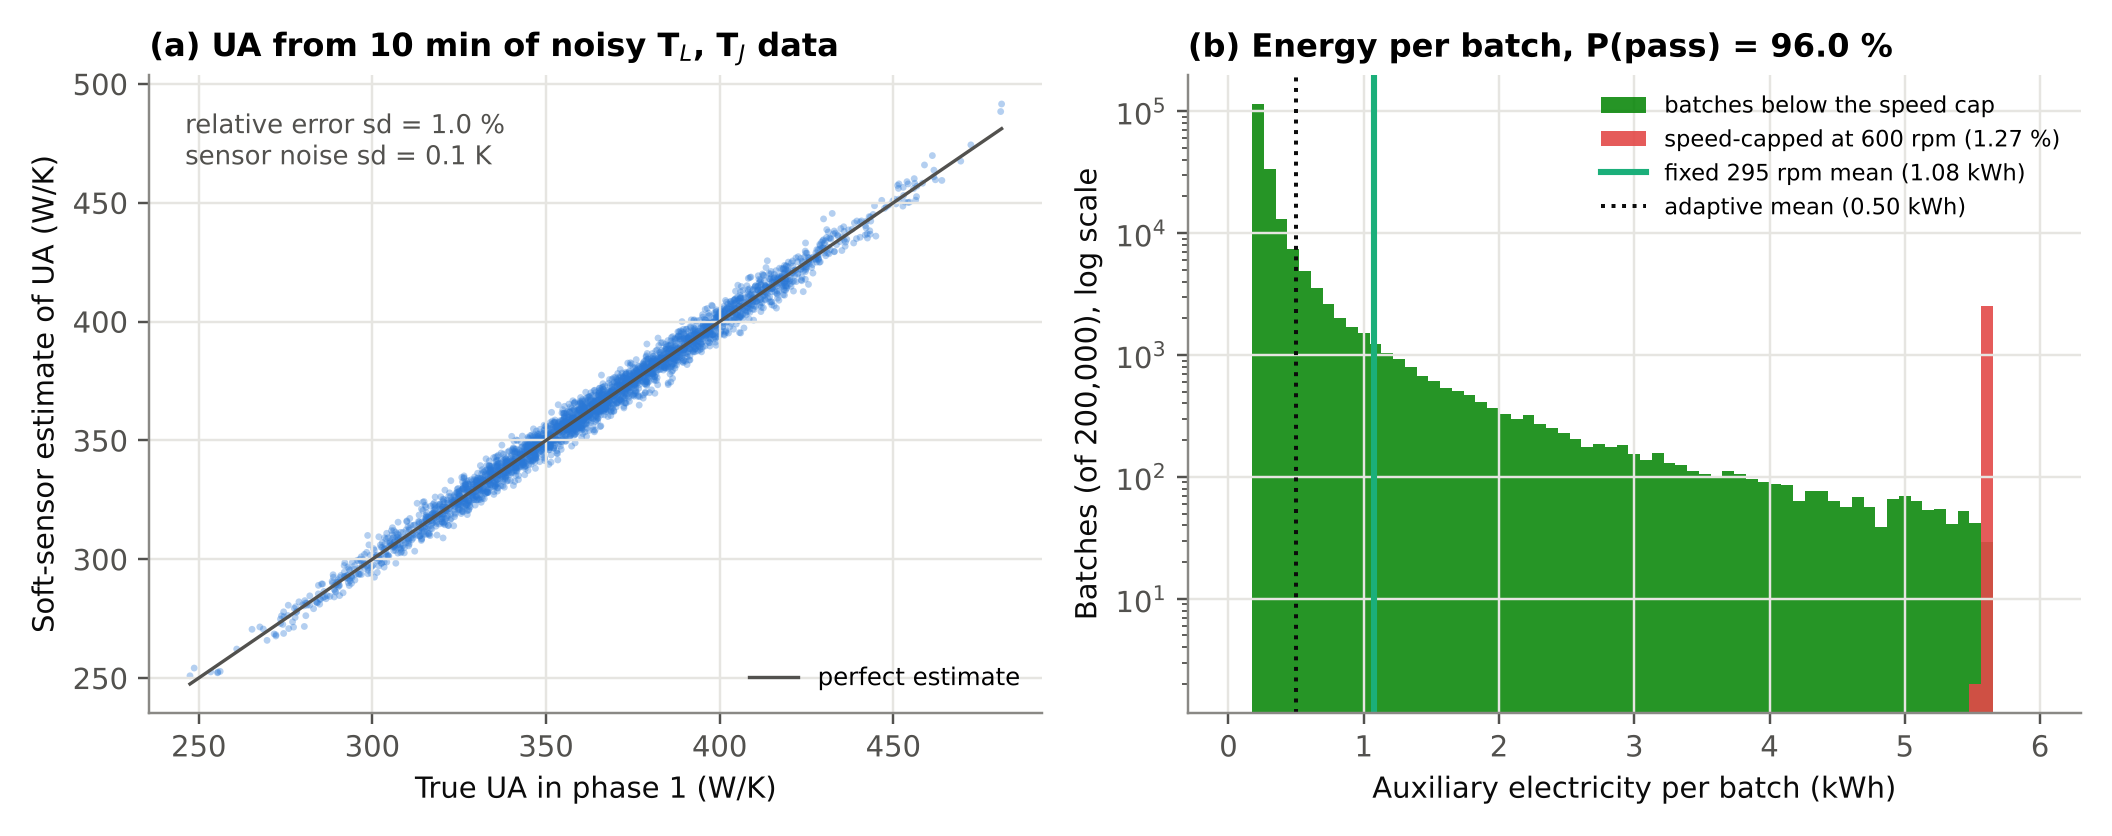
\includegraphics[width=0.82\textwidth]{adaptive_policy/adaptive_policy.png}
\caption{Adaptive policy: (a) soft-sensor estimate of \(UA\); (b) energy per batch, with speed-capped batches in red.}
\label{fig:adaptive}
\end{figure*}

\subsection{Model-form stress test}
The closure exponents cannot be given defensible probability distributions, so they were tested as scenarios. Film-coefficient scaling (\(h_i \propto N^{2/3}\)~\cite{b5}, \(h_o \propto \mdot^{\le 0.8}\)~\cite{b1}) bounds them by \(e_N/(2/3) + e_M/0.8 \le 1\). Varying the wall and fouling share of the total resistance gives the three closures in Table~\ref{tab:scen}. Under weak scaling no fixed setting within the bounds reaches 95\,\%. The adaptive policy degrades more than the fixed setting, because it extrapolates a speed change through \(e_N\). By contrast, splitting the jacket into 10 cells in series (towards plug flow) raises the recommended setting's pass rate from \vJetPassOne\,\% to \vJetPassTen\,\%, so the well-mixed jacket is the conservative limit.

\begin{table}[!t]
\centering
\caption{Pass probability of the fixed and adaptive designs under three heat-transfer closures (stress set)}
\label{tab:scen}
\footnotesize
\input{generated/tab_paper_scenarios.tex}
\end{table}

\section{Conclusion}
The coolant-side resistance is the physics missing from the original cooling model, and it reverses its conclusion. Under a physical pump limit and actual-flow energy accounting, the cheapest fixed setting with a validated 95\,\% reliability is \vRecRpm\ rpm at the maximum coolant flow, at \vRecE\ kWh per batch. A soft-sensor-based adaptive policy halves the expected energy in simulation. Both results depend on the assumed heat-transfer closure, so flow and speed step tests to identify \(U_{ref}\), \(e_M\) and \(e_N\) are the next step. The Python results and figures are reproducible from fixed seeds with one command.

\balance
\begin{thebibliography}{9}
\footnotesize
\bibitem{b1} T. L. Bergman, A. S. Lavine, F. P. Incropera, D. P. DeWitt, \emph{Fundamentals of Heat and Mass Transfer}, 7th ed. Wiley, 2011.
\bibitem{b2} A. Saltelli \emph{et al.}, ``Variance based sensitivity analysis of model output: design and estimator for the total sensitivity index,'' \emph{Comput. Phys. Commun.}, vol. 181, pp. 259--270, 2010.
\bibitem{b3} J. Luedtke and S. Ahmed, ``A sample approximation approach for optimization with probabilistic constraints,'' \emph{SIAM J. Optim.}, vol. 19, pp. 674--699, 2008.
\bibitem{b4} E. B. Wilson, ``Probable inference, the law of succession, and statistical inference,'' \emph{J. Amer. Statist. Assoc.}, vol. 22, pp. 209--212, 1927.
\bibitem{b5} T. H. Chilton, T. B. Drew, R. H. Jebens, ``Heat transfer coefficients in agitated vessels,'' \emph{Ind. Eng. Chem.}, vol. 36, pp. 510--516, 1944.
\bibitem{b6} C. Moler and C. Van Loan, ``Nineteen dubious ways to compute the exponential of a matrix, twenty-five years later,'' \emph{SIAM Rev.}, vol. 45, pp. 3--49, 2003.
\end{thebibliography}

\end{document}
